\begin{figure*}[hbtp]
  \centering
  \subfigure{
    \label{fig:louvainrak-sta--all}
    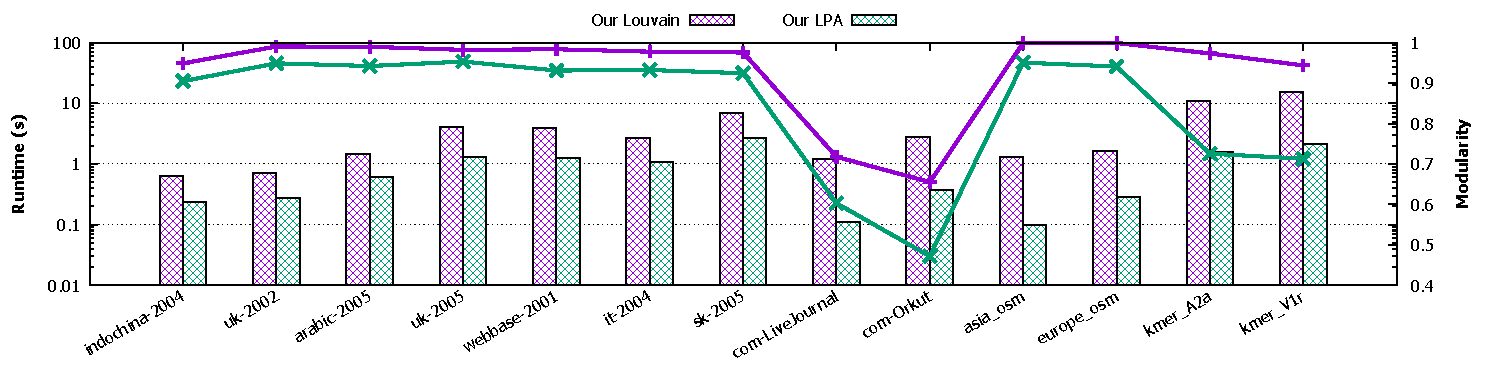
\includegraphics[width=0.98\linewidth]{out/louvainrak-sta.pdf}
  } \\[-2ex]
  \caption{Time taken (boxes), and modularity of communities obtained (lines) with our \textit{Louvain} and \textit{LPA} for each graph in the dataset. Runtime is shown with logarithmic scale on the left Y-axis (in seconds), and modularity is shown with linear scale on the right Y-axis.}
  \label{fig:louvainrak-sta}
\end{figure*}
